\chapter{統計モデル}
この章ではついにデータが登場する。データは母集団から無作為抽出によって得られた数値であるとする。
データを大文字の$X_1,X_2,\cdots,X_n$とし、モデルからサンプリングした確率変数を小文字の$x_1,x_2,\cdots,x_n$とする。
統計モデルはデータの出現頻度や統計量などの出現区間などを予測する。
まず、その予測可能なことについて列挙する。モデルとデータが異なる場合つまり、データの出現頻度をデータが予測できない場合に生じることについて説明する。

\section{正規分布を含んだ統計モデル}
次の3つを仮定したモデルを正規モデルと呼ぶ。
\begin{quote}
    \begin{enumerate}[(1)]
    \item 独立同分布
    \item その分布は、正規分布
    \item 正規分布の母数(平均と分散)はそれぞれ$\mu,\sigma^2$。
    \end{enumerate}
\end{quote}
この正規モデルを$M(\mu,\sigma^2)$と書く。$\sigma^2$をある特定の値にしたときのモデルを$M(\mu)$とし、$\mu$を特定の値にしたモデルを$M(\sigma^2)$とする。モデルに対してある特定の値を当てはめることができるのは、推測したい母集団について、すでに標本を得て、標本分布がわかっている場合である。この母集団を細分化した母集団について、推測した母数を使ったモデルで推測しても良いかを検討するときに、元の母集団に関する知識を使う。

%\subsection{最尤推定量を使ったモデル}
母集団から無作為抽出した標本(データの入った集合)を元にモデルを構築する。具体的には、$\mu_{ML}=\bar{X},\sigma^2_{ML}=\frac{1}{n}\sum(X_i-\bar{X})$とし、統計モデル$M(\mu_{ML},\sigma^2_{ML})$を最尤モデルと呼ぶ。

\begin{SMbox}{最尤モデルが最も良い予測をするかはわからない}
赤池も、最尤推定量がデータを推測する上で良い推定量になっているかの根拠にならないことを指摘している\ref{1570854174583769344}。
    \begin{quote}
    R.A.Fisherの研究により、観測データxが実際に$p(x|a)$の形の確率分布に従って発生するとき、最尤法が優れた特性を示すことが示された。しかし、応用の場面では、データを生み出す確率的な構造が完全に分かっていることは無いから、Fisherの議論は、最尤法の実上用の根拠を与えない。
    \end{quote}
\end{SMbox}

以下では、$M(\mu)$による予測について説明する。

\if 0 

\fi

\if 0

\fi

\subsection{データが出現しやすい区間}
ある決められた確率でデータが出現するとモデルが予測する区間を予測区間という。
割合として、よく使われる$95\%$を設定したものを$95\%$予測区間という。
正規分布を含んだモデル$M(\mu)$において、予測区間は比較的簡単に求めることができる。
具体的には、正規分布の規格化を行い、標準正規分布に従うように変換を行い、$\frac{x-\mu}{\sigma}$であるので、予測区間は、
\begin{eqnarray*}
    %-z_{0.05} <\frac{x-\mu}{\sigma} <z_{0.05} \\
    \mu-z_{0.05}\sigma < x < \mu+z_{0.05}\sigma
\end{eqnarray*}
である。この範囲に$95\%$のデータが生じることをモデルが予測する。実際にそのようになるかは不明であり、予測であることを意識した方が良い。

$68\%$の確率でデータを含むと予測する区間が求められる。
\begin{eqnarray*}
    %-z_{0.05} <\frac{x-\mu}{\sigma} <z_{0.05} \\
    \mu-\sigma < x < \mu+\sigma
\end{eqnarray*}

\subsection{母集団の標本が指数分布的に分布していた場合}
母集団の分布形と統計モデルに含まれている確率分布関数が著しく異なる場合を考える。
母集団分布として、指数分布を仮定しする。これは、自然から指数分布的なデータが得られたときのことを想定している。
これを予測するモデルを正規分布の仮定されたモデルとする。

最尤モデルは、$M(\mu_{ML},\sigma^2_{ML})$である。ここから、
\begin{eqnarray*}
    %-z_{0.05} <\frac{x-\mu}{\sigma} <z_{0.05} \\
    \mu_{ML}-\sigma_{ML} < x < \mu_{ML}+\sigma_{ML}
\end{eqnarray*}
が$68\%$予測区間になる。
言い換えれば、標準偏差の間に、サンプルの平均が入る確率が$68\%$であることをモデルが予測している。
このことを数値シミュレーションにより確かめる。
指数分布からランダムサンプリングを行い、無作為抽出によりサンプルサイズ$10^6$の標本を得たとする。
サンプルが上記の区間に入っている割合を計算する。

\begin{lstlisting}
N = 10**6
sample = expon.rvs(scale=10,size=N)
#sample = norm.rvs(loc=0,scale=1,size=N)
lambd= np.average(sample)
print(np.average(sample),np.std(sample),np.var(sample))

mu = np.average(sample)
s = np.std(sample)

a,b = mu-s,mu+s
len(sample[np.where( (sample >a) & (sample<b) )])/N
\end{lstlisting}
この結果、期待していた値$68\%$よりも著しく大きな確率$86\%$程度を得る。
これは、モデルでは、正規分布を仮定していたが、実際には指数分布的なデータだったために生じる予測の間違いである。
以上でわかるのは、統計モデルと実際の母集団が乖離している場合には、標準誤差に間違いが多くなるということである。

\subsubsection{エラーバー(SD)から読み取れること}
正規分布と指数分布それぞれからサンプルサイズ$N=100$の標本を作り、プロットした(図\ref{fig:sample_norm_expon_model})。それぞれの分布の右側のエラーバーは、$68\%$予測区間。
標本が正規分布であるときには、$68\%$予測区間の中におよそ$68\%$のデータが含まれている。
一方で、標本が指数分布であるときは、モデルの予測と乖離する。このことは、図から読み解くことが難しい。

エラーバー(SD)だけが描かれた図を見るとデータに対する印象が変わる(図\ref{fig:model_predict_SD})。
図\ref{fig:model_predict_SD}には、正規分布と指数分布から得られた標本から、最尤推定を行ったモデル$M(\mu_{ML},\sigma^2_{ML})$における$68\%$予測区間を描画している。
データが正規分布的であるならば、データが区間に入っている割合が予測と一致する。
一方で、データが指数分布的であるならば、モデルの予測(エラーバー)から得られることと、実際のデータは乖離する。
エラーバーからは、中央からデータが対称に分布しており、その中に、$68\%$のデータが入っていることを我々は読み取ろうとする。
データのばらつきを表すためにSDを描いた場合、それが正規分布的な標本でない限り、データのばらつきの意味が伝わりにくくなる。
%実際のデータは図\ref{fig:sample_norm_expon_model}にある通りであり、モデルの予想とは一致しない。
%エラーバーにSDを描くときには、特に指定がない限り、正規分布を仮定したモデルを想定しているということを想定し、その中におよそ$68\%$のデータが入るということを示すという意図がある。

実際の研究活動において、モデルを考えてエラーバーにSDを書いていると断言しがたい。
例えば、SDが描かれているのに、検定においては正規分布を仮定しない統計モデルを使っていることが多々ある。
これは、データの描画においては、正規分布を仮定しているにもかかわらず、仮説検定においては正規分布をもとにした推測をやめていることを意味する。
この場合、著者が何を考えてSDを描いたのかを判断することが難しくなる。
%また、データが正規分布的であることに確信を得ることは、サンプルサイズを大きくした標本から想像するしかなく、費用がかさむので行われない。
%このこと、モデルの予測が当たることを肯定できる根拠がないことを意味する。

測定の精度の良さを示す指標としてSDを書くことがある。この場合、ただ単にSDが小さければ良い計測であることを示す意図がある。
%データが正規分布であるという強い前提がある。

\begin{figure}
    \begin{center}
        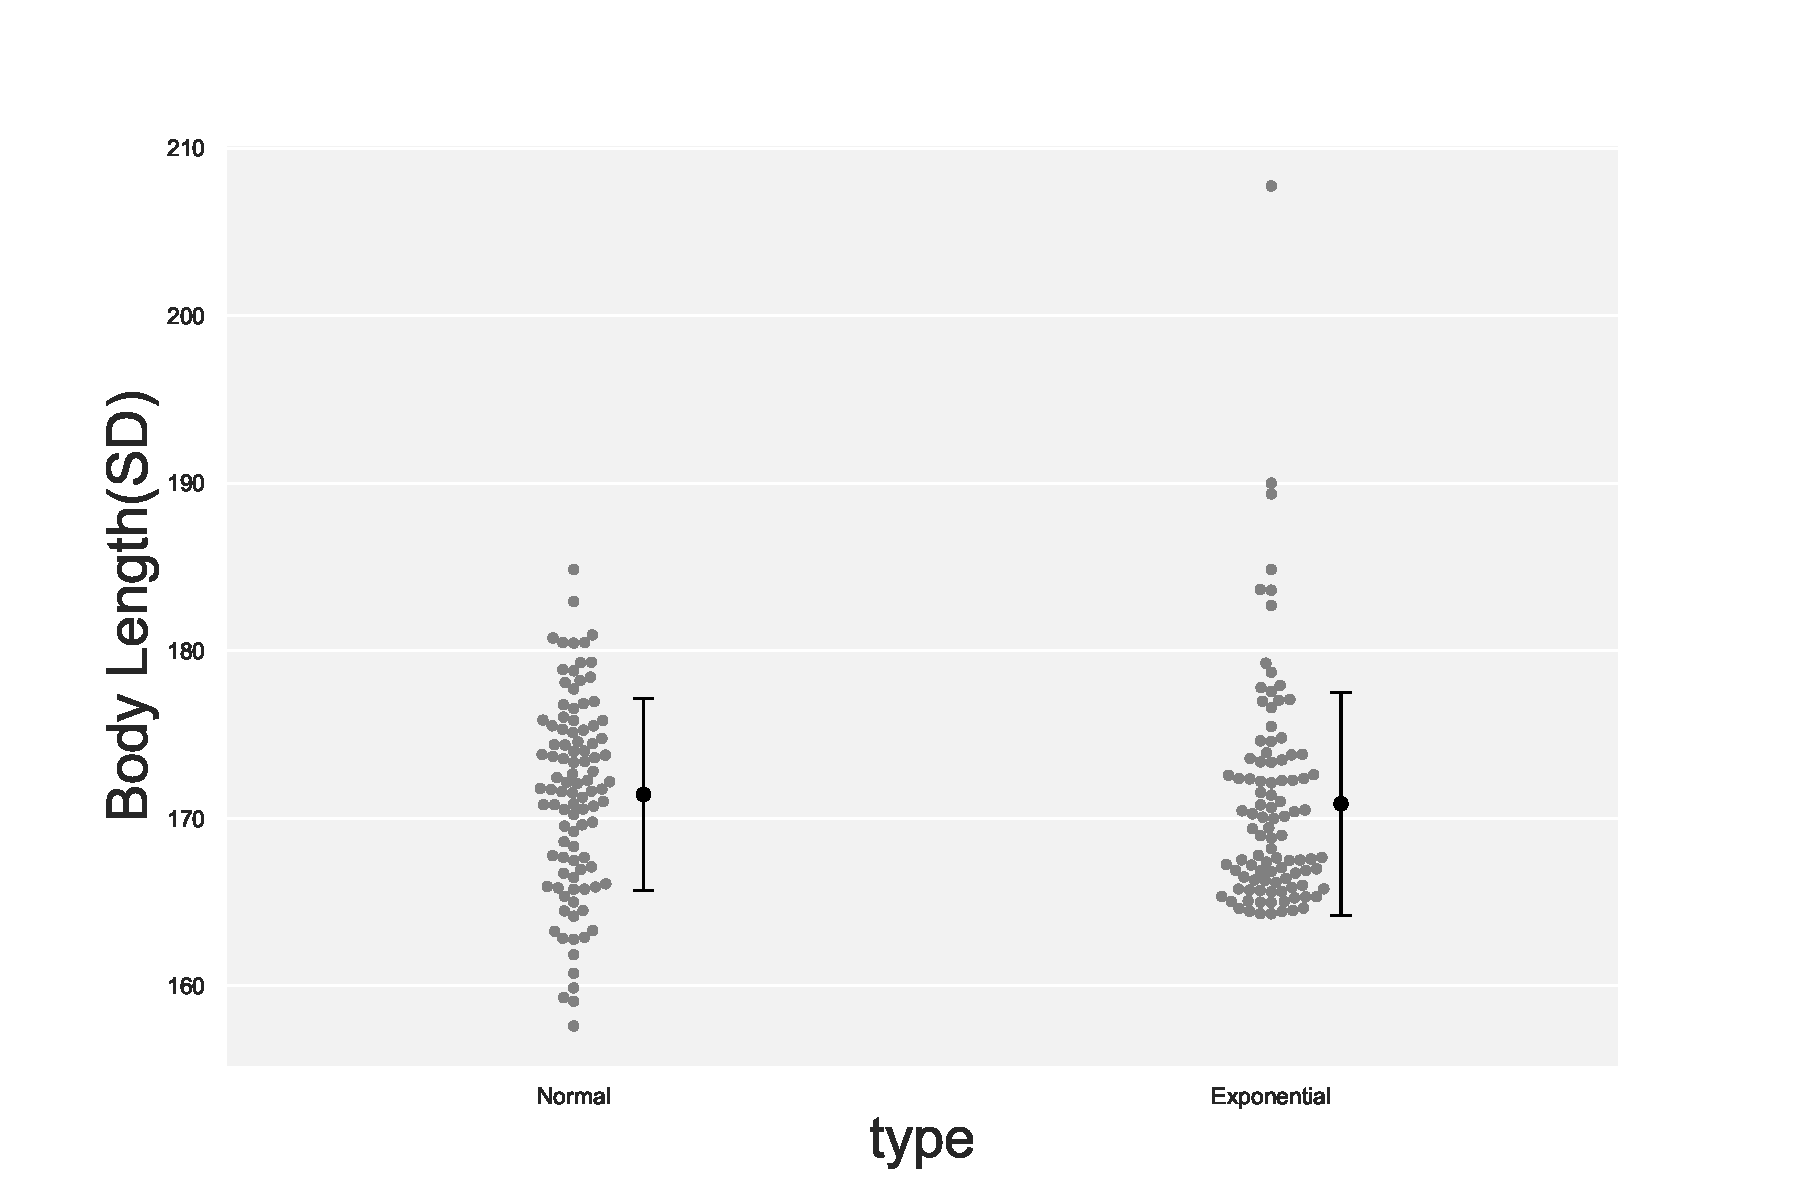
\includegraphics[width=15cm]{./image/12_/sample_norm_expon.pdf}
        \label{fig:sample_norm_expon_model}
        \caption{正規分布と指数分布それぞれからサンプルサイズ$N=100$の標本をプロットした。それぞれの右側にあるエラーバーは、正規分布モデルが予測した$68\%$予測区間。}
      \end{center}
    \end{figure}


\begin{figure}
    \begin{center}
        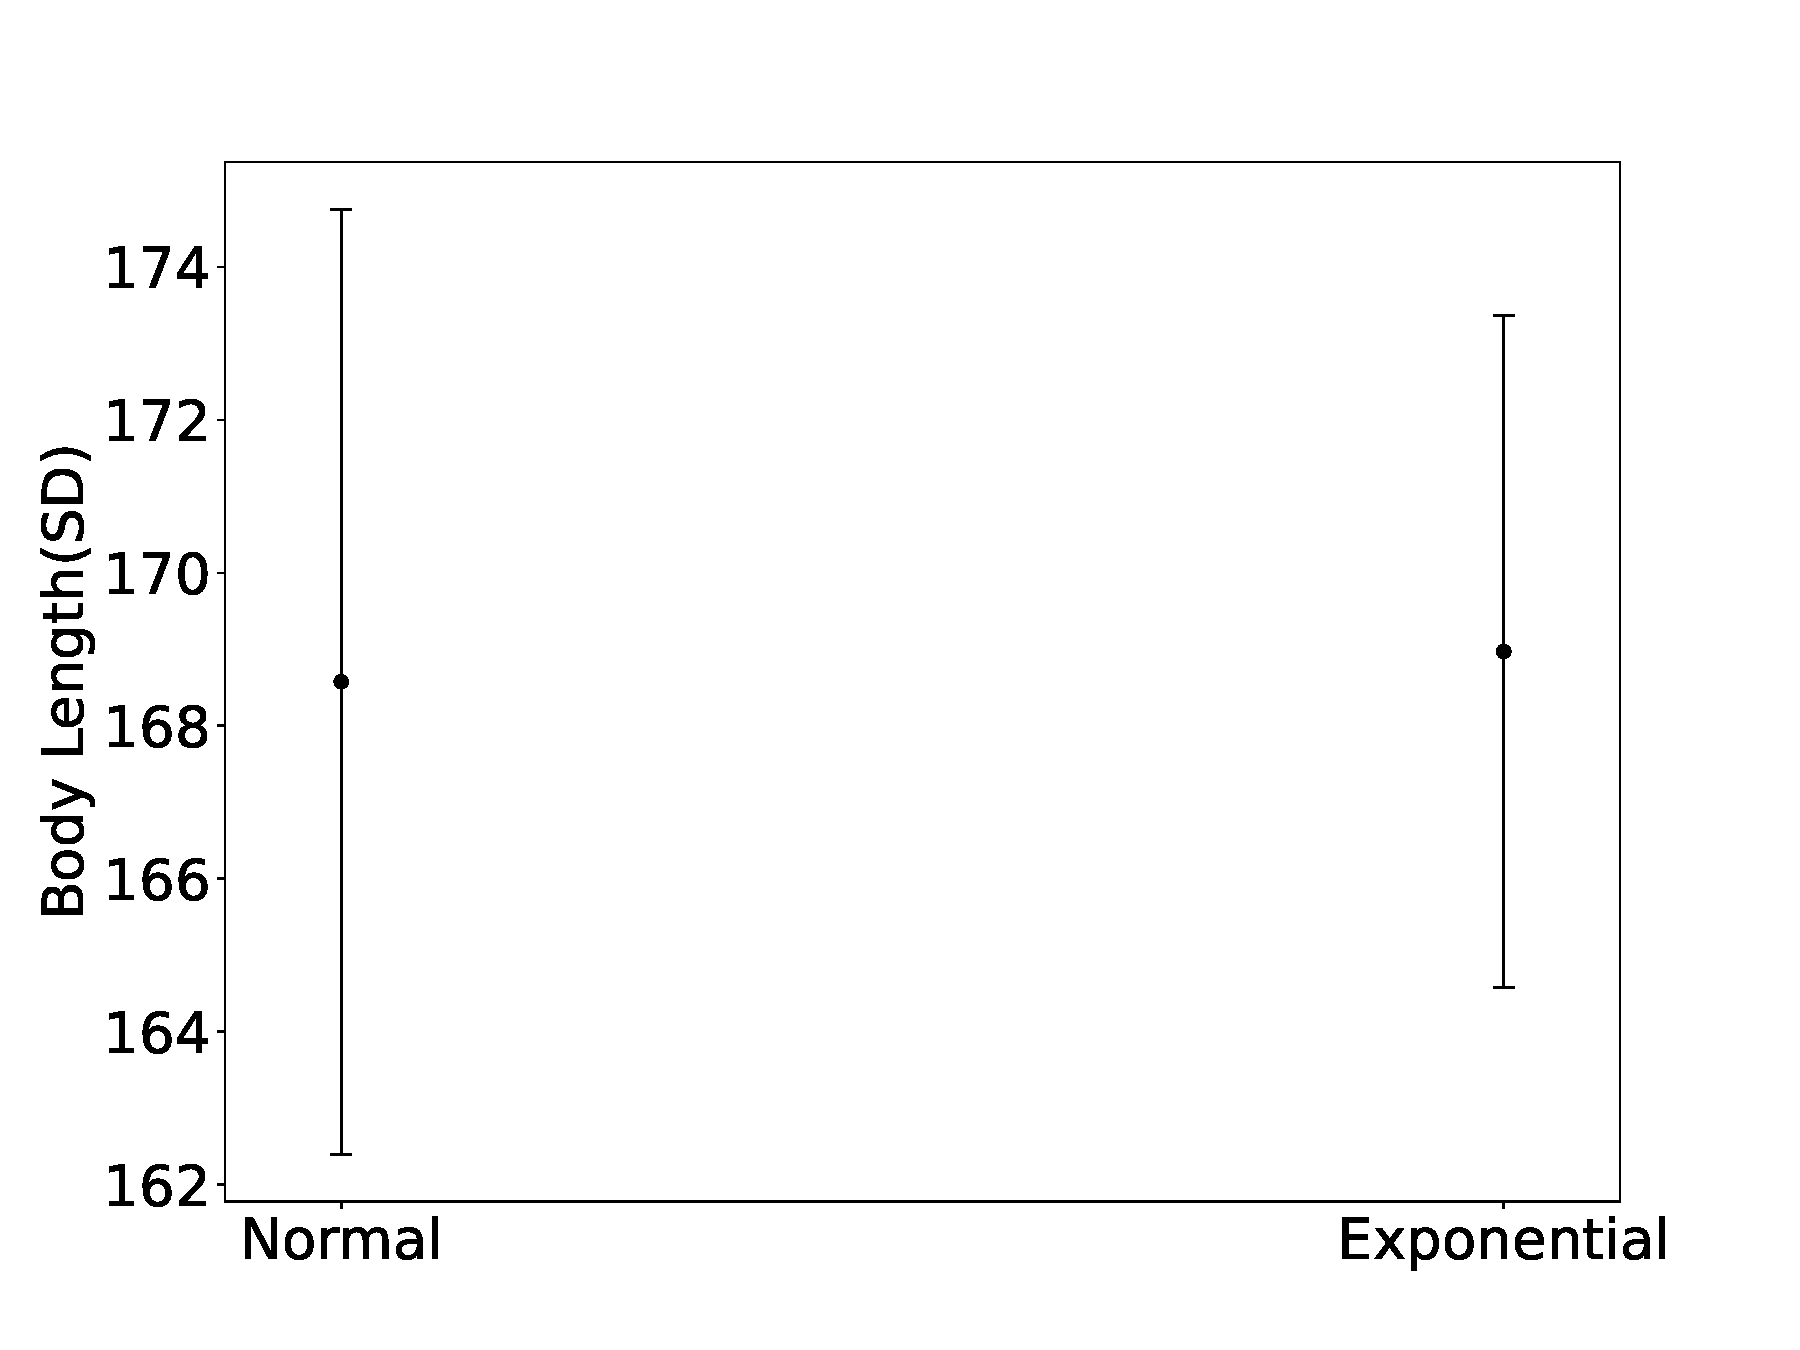
\includegraphics[width=15cm]{./image/12_/model_predict_SD.pdf}
        \label{fig:model_predict_SD}
        \caption{正規分布と指数分布それぞれからサンプルサイズ$N=100$の標本を得た。その標本から推測される$68\%$予測区間を描画した。}
      \end{center}
    \end{figure}

    

\subsection{平均値が出現する区間}
統計モデル$M(\mu)$では、標本の平均値$\bar{x}$が、以下の区間で$95\%$の確率で見つかる。
\begin{equation*}
    \mu - z_{0.025} \frac{\sigma}{\sqrt{n}} < \bar{X} < \mu + z_{0.025} \frac{\sigma}{\sqrt{n}}
\end{equation*}
%$Z(\bar{x},\mu)$が$N(0,1)$に従うということから、$Z(\bar{X},\mu)$が$N(0,1)$における出現頻度が計算できる。
この統計モデルからサンプリングした標本の標本平均$\bar{x}$が$95\%$の確率で見つかる範囲のことを$95\%$信頼区間という。これも、モデルの予測である。

一般的な定義として、要約統計量($\bar{x}$など)が$95\%$の確率で見つかることを予測する最小の区間を信頼区間という。



\if 0
 川久保統計学P.166
 \fi


%![Z値の頻度]()

信頼区間の中に標本平均が含まれていることは、標本がモデルにり推測可能であることの証拠の一つになる。
ただし、予測可能かの判断には、複合的に指標を見る必要がある。
%$\bar{X}$が$95\%$信頼区間の中に入っていることは、この統計モデル
%信頼区間の中に統計量があれば、
%このことから、統計モデル$M(\mu)$でサンプリングしたときに、$95\%$の確率で、この範囲に平均値$\bar{X}$がえられます。


%標本$1$標本$2$について、これを計算してみる。平均値は、それぞれ172.4, 169.0です。
%\subsection{複数の確率変数から推測する}




\section{指数分布を含んだ統計モデル}
\begin{quote}
    \begin{enumerate}[(1)]
    \item 独立同分布
    \item その分布は、指数分布$(\lambda\exp{(-\lambda x)})$
    \item 指数分布の母数は$\lambda$
    \end{enumerate}
\end{quote}
このモデルを$M_E(\lambda)$とする。
このモデルの$95\%$予測区間は、
\begin{equation*}
    \frac{1}{\lambda} \log\frac{1}{1-\alpha/2} ,\frac{1}{\lambda}\log\frac{\alpha}{2}    
\end{equation*}
である。
%指数モデルにおける$95\%$予測区間は、構成が難しいようなので、省略する\footnote{どうすれば求められるのか、わからない}。
$95\%$信頼区間は式\ref{exp_model_confidence_interval}である。


\subsection{信頼区間を近似する}
$95\%$信頼区間(式\ref{exp_model_confidence_interval})を近似的に求める方法がある。
中心極限定理を使う。このモデルでは、サンプルの平均および分散は、$E[x]=\frac{1}{\lambda},Var[x]=\frac{1}{\lambda^2}$である。このとき、中心極限定理により、$\bar{x}\sim N(E[x],Var[x]/n)$である。よって、$95\%$信頼区間は、
\begin{equation*}
    \frac{1}{\lambda}-z_{0.05}\frac{1}{\sqrt{n}\lambda}<\bar{x}<\frac{1}{\lambda}+z_{0.05}\frac{1}{\sqrt{n}\lambda}
\end{equation*}
である。

解析的に求めた信頼区間と中心極限定理による近似的な信頼区間を比較する(図\ref{fig:model_predict_CI_interval})。
$\lambda=10$としたので、平均は全て$10$である。
$N$が小さいと、解析と近似での信頼区間に差が生じている。近似的な信頼区間は、$0$よりも小さな値も出現することを予測している。平均$10$の指数モデルでは、平均が$0$以下になることはない。このように、モデルの想定しない区間も信頼区間に含めている。
$N$が大きくなると、解析と近似での信頼区間の違いは少なくなる。これは、中心極限定理の帰結から当然である。

\begin{figure}
    \begin{center}
        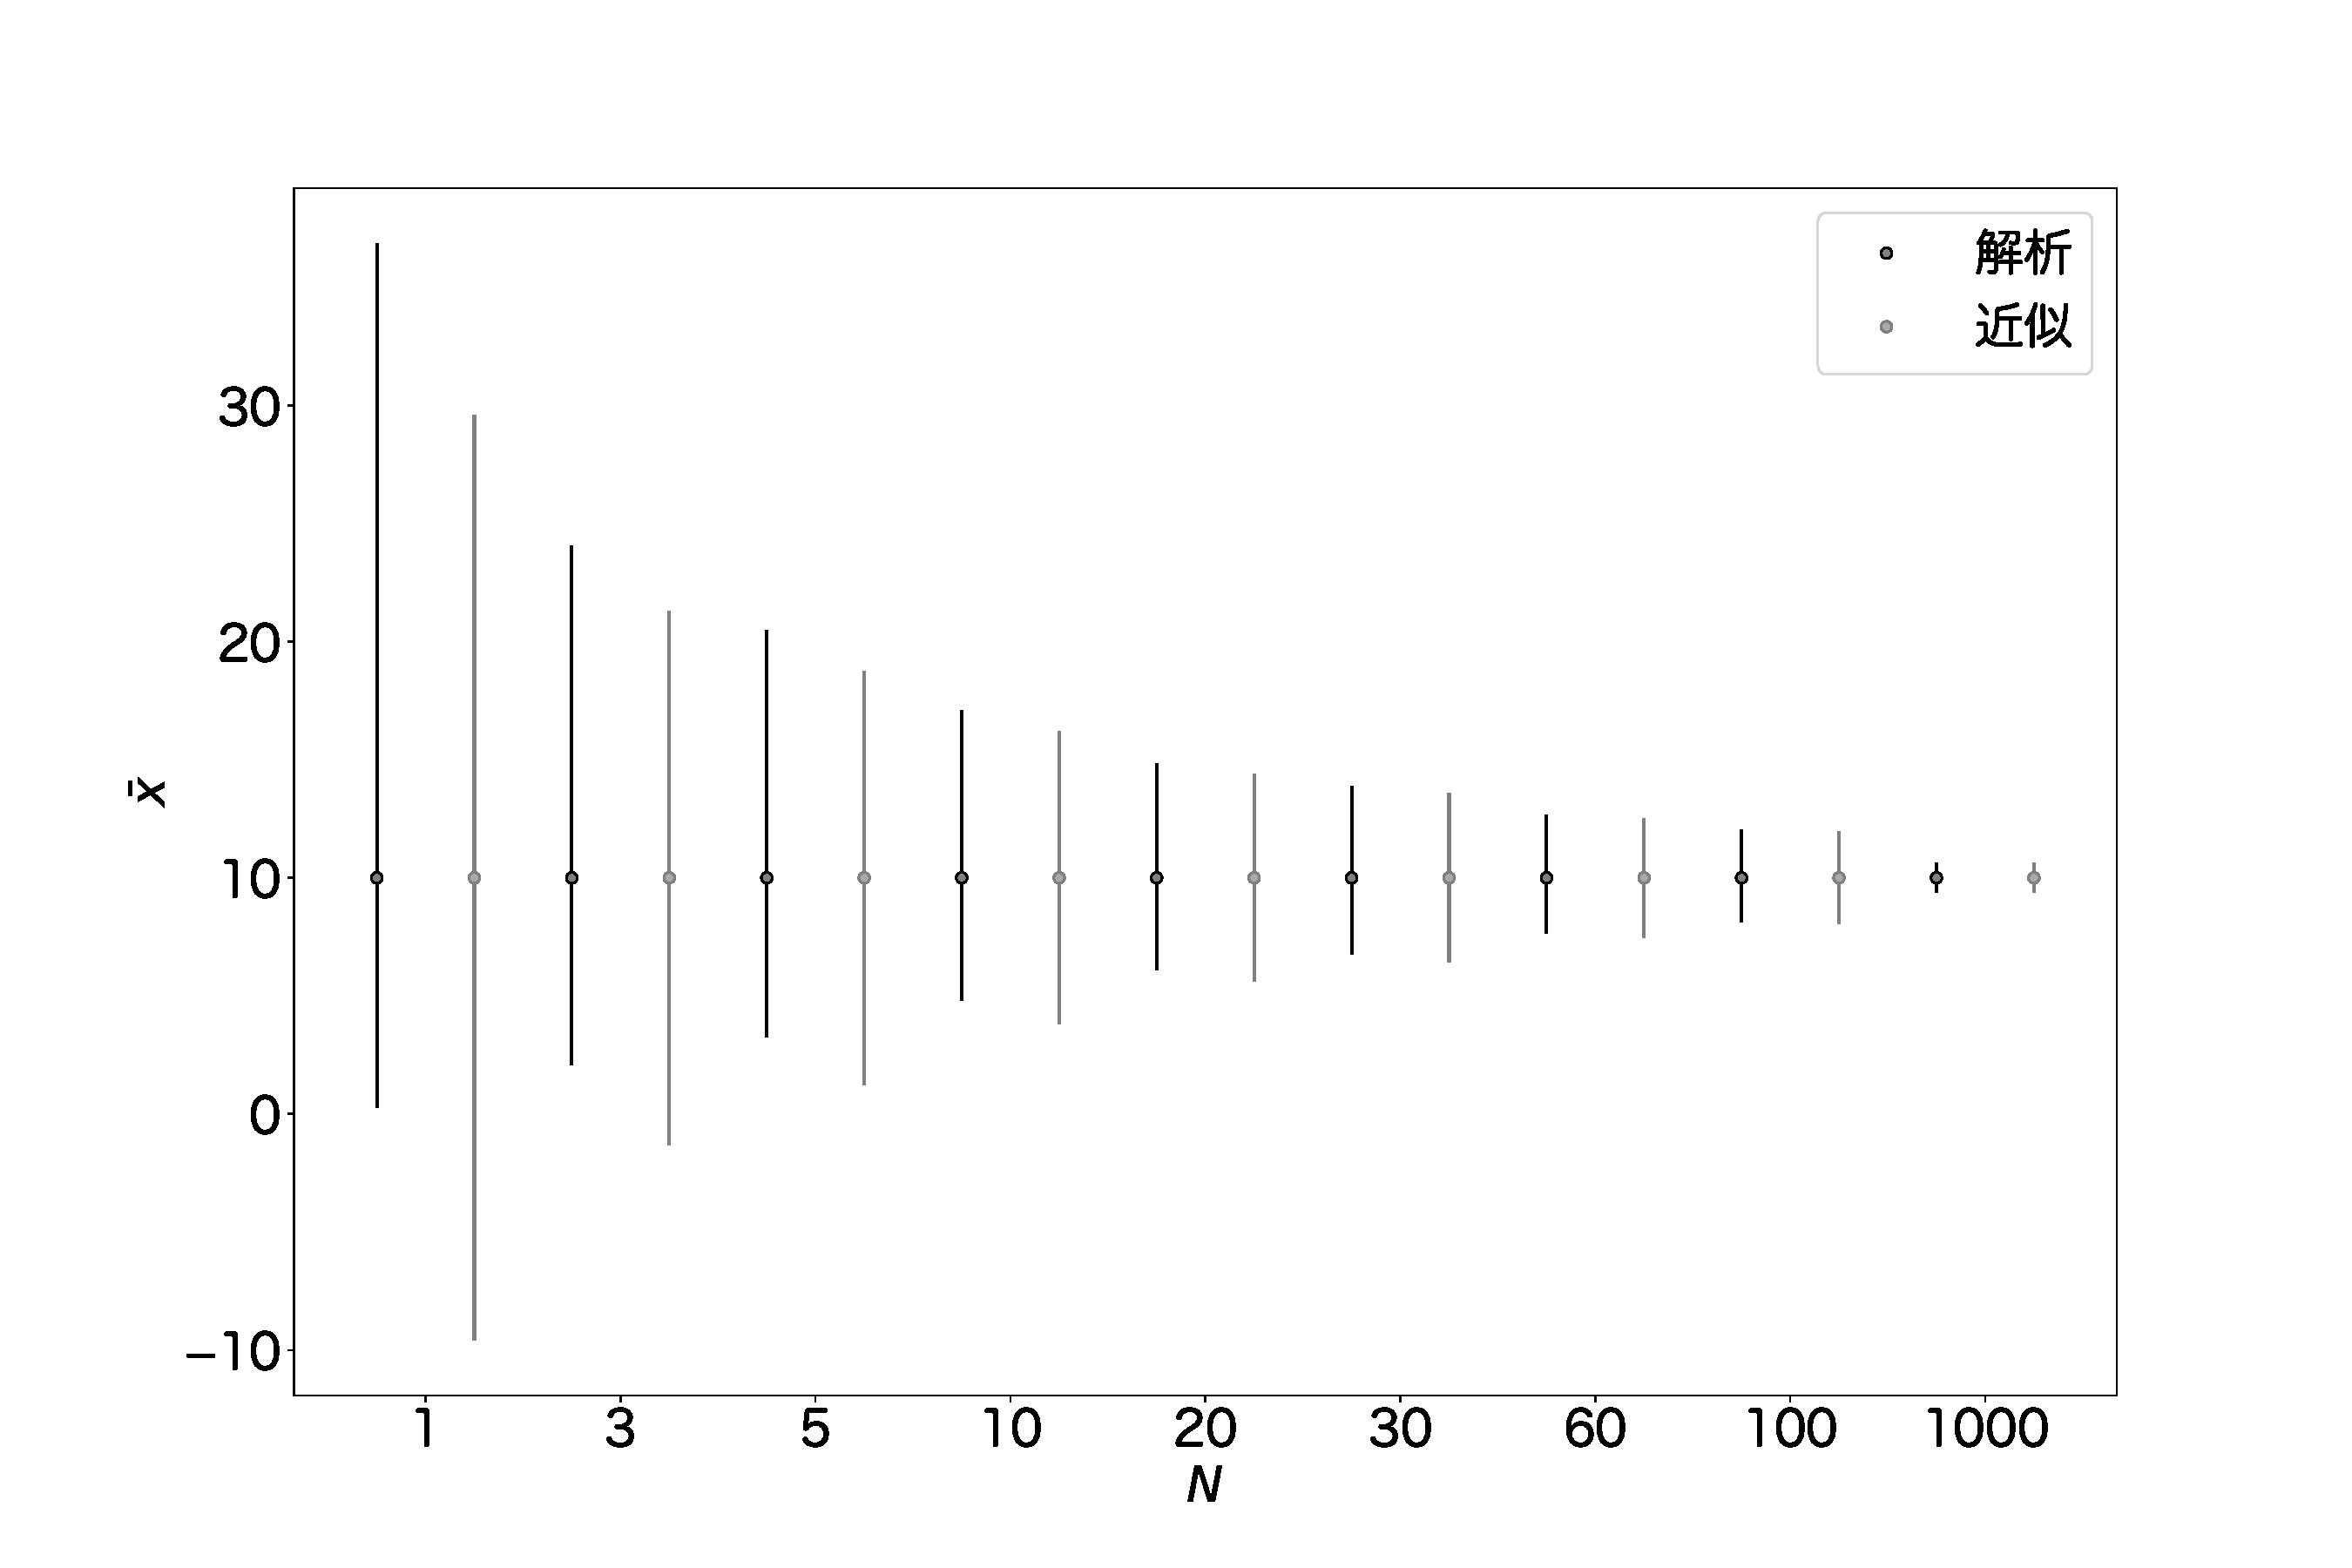
\includegraphics[width=15cm]{./image/12_/confidence_expon_interval.pdf}
        \label{fig:model_predict_CI_interval}
        \caption{解析的な信頼区間と近似によって求められた信頼区間。$1/\lambda=10$とする。横軸にサンプルサイズ。縦軸に、平均値。エラーバーは信頼区間(CI)。}
      \end{center}
    \end{figure}

\section{モデルの選択}
データの分布とモデルの分布が一致しているとき、そのモデルの予測も当たりやすい。
例えば、データがある値の周りに対象に分布していないにもかかわらず、正規モデルを使うと、その予想は当たりにくい。
モデルの予測が当たると思わせるには、標本分布に関する知識が必要であり、その知識があれば、モデルの予測が当たりやすいと他の人に説得しやすくなる。
このことから、まず、標本分布に関する、適当な分布の形(母数を含めた)を探索する必要がある。
モデルを選択できるほどのサンプルサイズを集めて、母集団を予測しやすいモデルを決めることで、予測が当たりやすくなり、モデルの予測を信頼しやすくなる。

実際の研究では、実験のコスト増加のことを考慮すると、事前実験により標本分布を調べることは、ほとんど不可能である。
そこで、何も事前研究がないなら正規モデルにより推測を行うことを検討するのも良い。
モデルがデータを捉えていない場合でも、中心極限定理により信頼区間はそれなりに当たることが多い。
ただし、予測区間が現実をよく捉えているかはわからない。


%実験前の事前計画によって決めたモデルを、実験データを見た後に変更することは行ってはいけないことになっている。

%ここで、現状のデータからモデルを選択したとして、その予測が当たるかはわからない。
%サンプルサイズが小さいとき、予測が当たりそうなモデルを選ぶことが難しい。
%事前実験やこれまでの研究結果から推測し、モデルの分布と標本分布が一致していそうなモデルを選ぶことになる。

\subsection{累積分布によるデータとモデルの比較}

標本の累積分布のプロット方法について説明する。
標本$X_1,X_2,\cdots,X_n$を小さいものの順に並び替えたものを、$X_{r(1)},X_{r(2)},\cdots,X_{r(n)}$とする。ここで、$r(j)$は、$j$番目のデータのインデックスを返す関数である。
そして、
\begin{equation*}
    (X_{r(j)},j/n) \ \ \ (j=1,2,\cdots,n)
\end{equation*}
をプロットする。
言い換えれば、累積分布は、標本を小さい順に並べたものと、順位をサンプルサイズで割ったもののペアをプロットしたものである。

具体的なコードは次のようになる
\begin{lstlisting}
def cummlative_norm(data):
    sorted_data = np.sort(data) # 順番の並び替え X_{r(j)}
    x = np.arange(len(data))/len(data) # データ数分のj/n 
    mu_ml,sigma_ml = np.mean(data),np.std(data)
    predict_cdf = norm(mu_ml,sigma_ml).cdf(sorted_data)
    return sorted_data,x,predict_cdf
\end{lstlisting}

\subsubsection{累積分布の傾き}
累積分布は、データの密集度が高い範囲において、傾きが大きくなり、密集度の小さい範囲では、傾きが小さくなる(図\ref{fig:qq_ccummlative_data_example_normummlative})。


\begin{figure}
    \begin{center}
        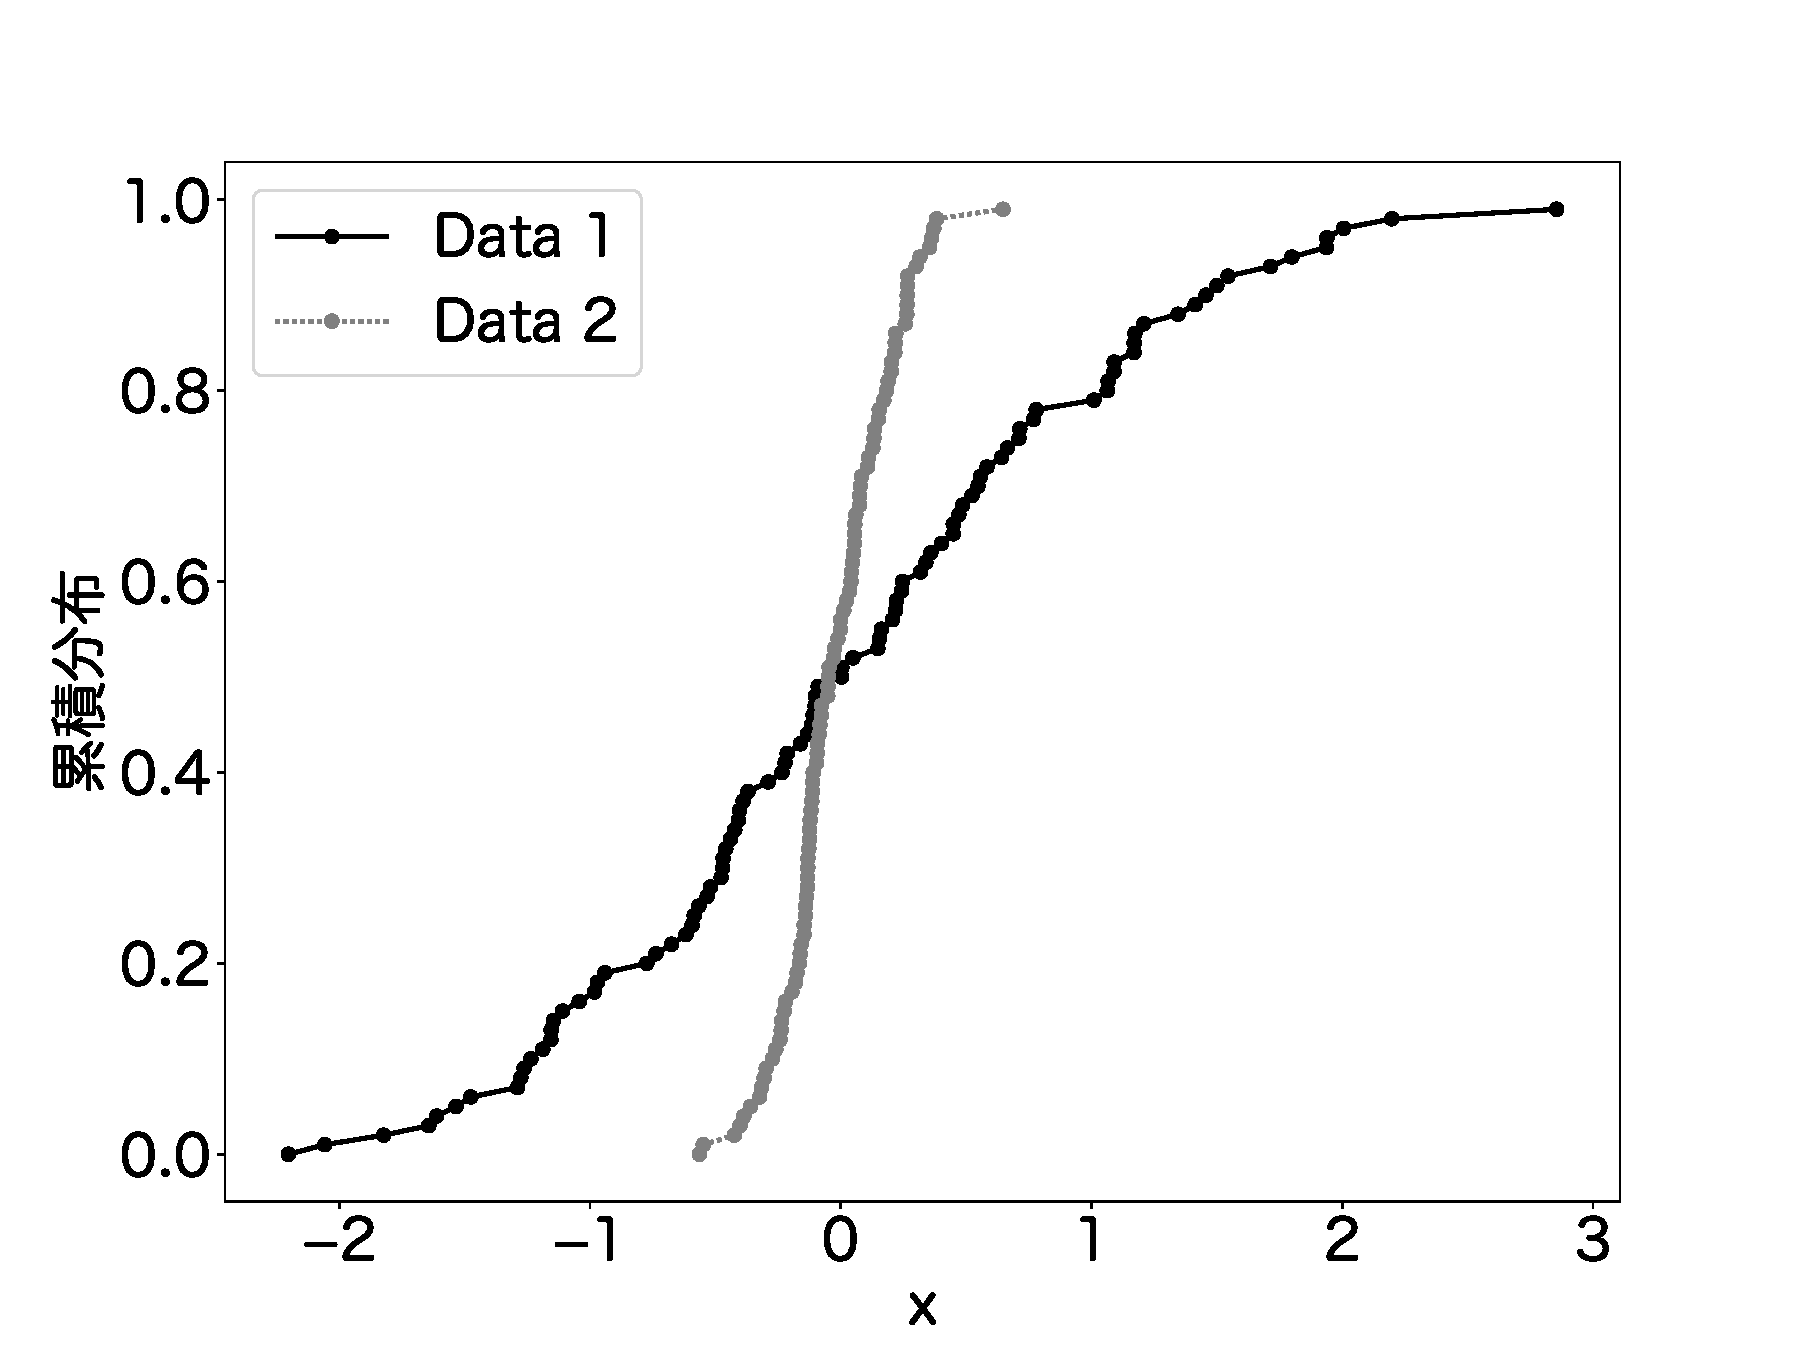
\includegraphics[width=7.5cm]{./image/12_/cummlative_data_example_norm.pdf}
        \label{fig:qq_ccummlative_data_example_normummlative}
        \caption{データの累積分布。Data 1は、正規分布$N(0,1)$、Data 2は正規分布$N(0,0.2)$からサンプリングした。サンプルサイズは$100$}
    \end{center}
\end{figure}


\subsubsection{データとモデルの比較}
図\ref{fig:qq_cummlative_30}図\ref{fig:qq_cummlative}右側に累積分布を描いておいた。
データは、(a)正規分布、(b)指数分布、(c)ガンマ分布からそれぞれサンプルサイズ$100$の標本である。
それぞれに、正規分布の最尤モデルを重ね書きしておいたので、最尤モデルとの乖離具合が把握できる。
(a)では、最尤正規モデルとデータが一致している。
(b,c)では、最尤正規モデルの曲線上に、データの累積分布の点が乗っていないので、モデルとデータが乖離していることが示唆される。
このことから、このようなデータが得られたなら、モデルを再構築したほうが良い。
また、サンプルサイズを30にした図\ref{fig:qq_cummlative_30}では、データが正規分布であっても、正規モデルによって推測することが良いのかはぱっと見では判断しにくく、正規モデルを確信を持って利用しにくくなる。

\subsection{qqプロットによるデータと正規分布の比較}
qqプロットについて説明する。
まず上記、$(X_{r(j)},j/n)$について、$j/n$を、$F^{-1}(j/n)$によって変換する。ここで、累積標準正規分布の逆関数を$F^{-1}(p)$とする。
つまり、
\begin{equation*}
(F^{-1}(j/n),X_{r(j)}) \ \ (j=0,1,\cdots,n)
\end{equation*}
をプロットする。



\begin{lstlisting}
    def qq_plot(data,ax):
        sorted_data = np.array(sorted(data))
        p = np.arange(len(data))/len(data)
        x_ = norm(0,1).ppf(p)
        return np.c_[x_,sorted_data]
\end{lstlisting}


qqプロットを図\ref{fig:qq_cummlative_30}図\ref{fig:qq_cummlative}左側に描いておいた。直線に乗っているデータは、正規モデルの推測が当たりやすいと考えられる。

\begin{figure}
    \begin{center}
        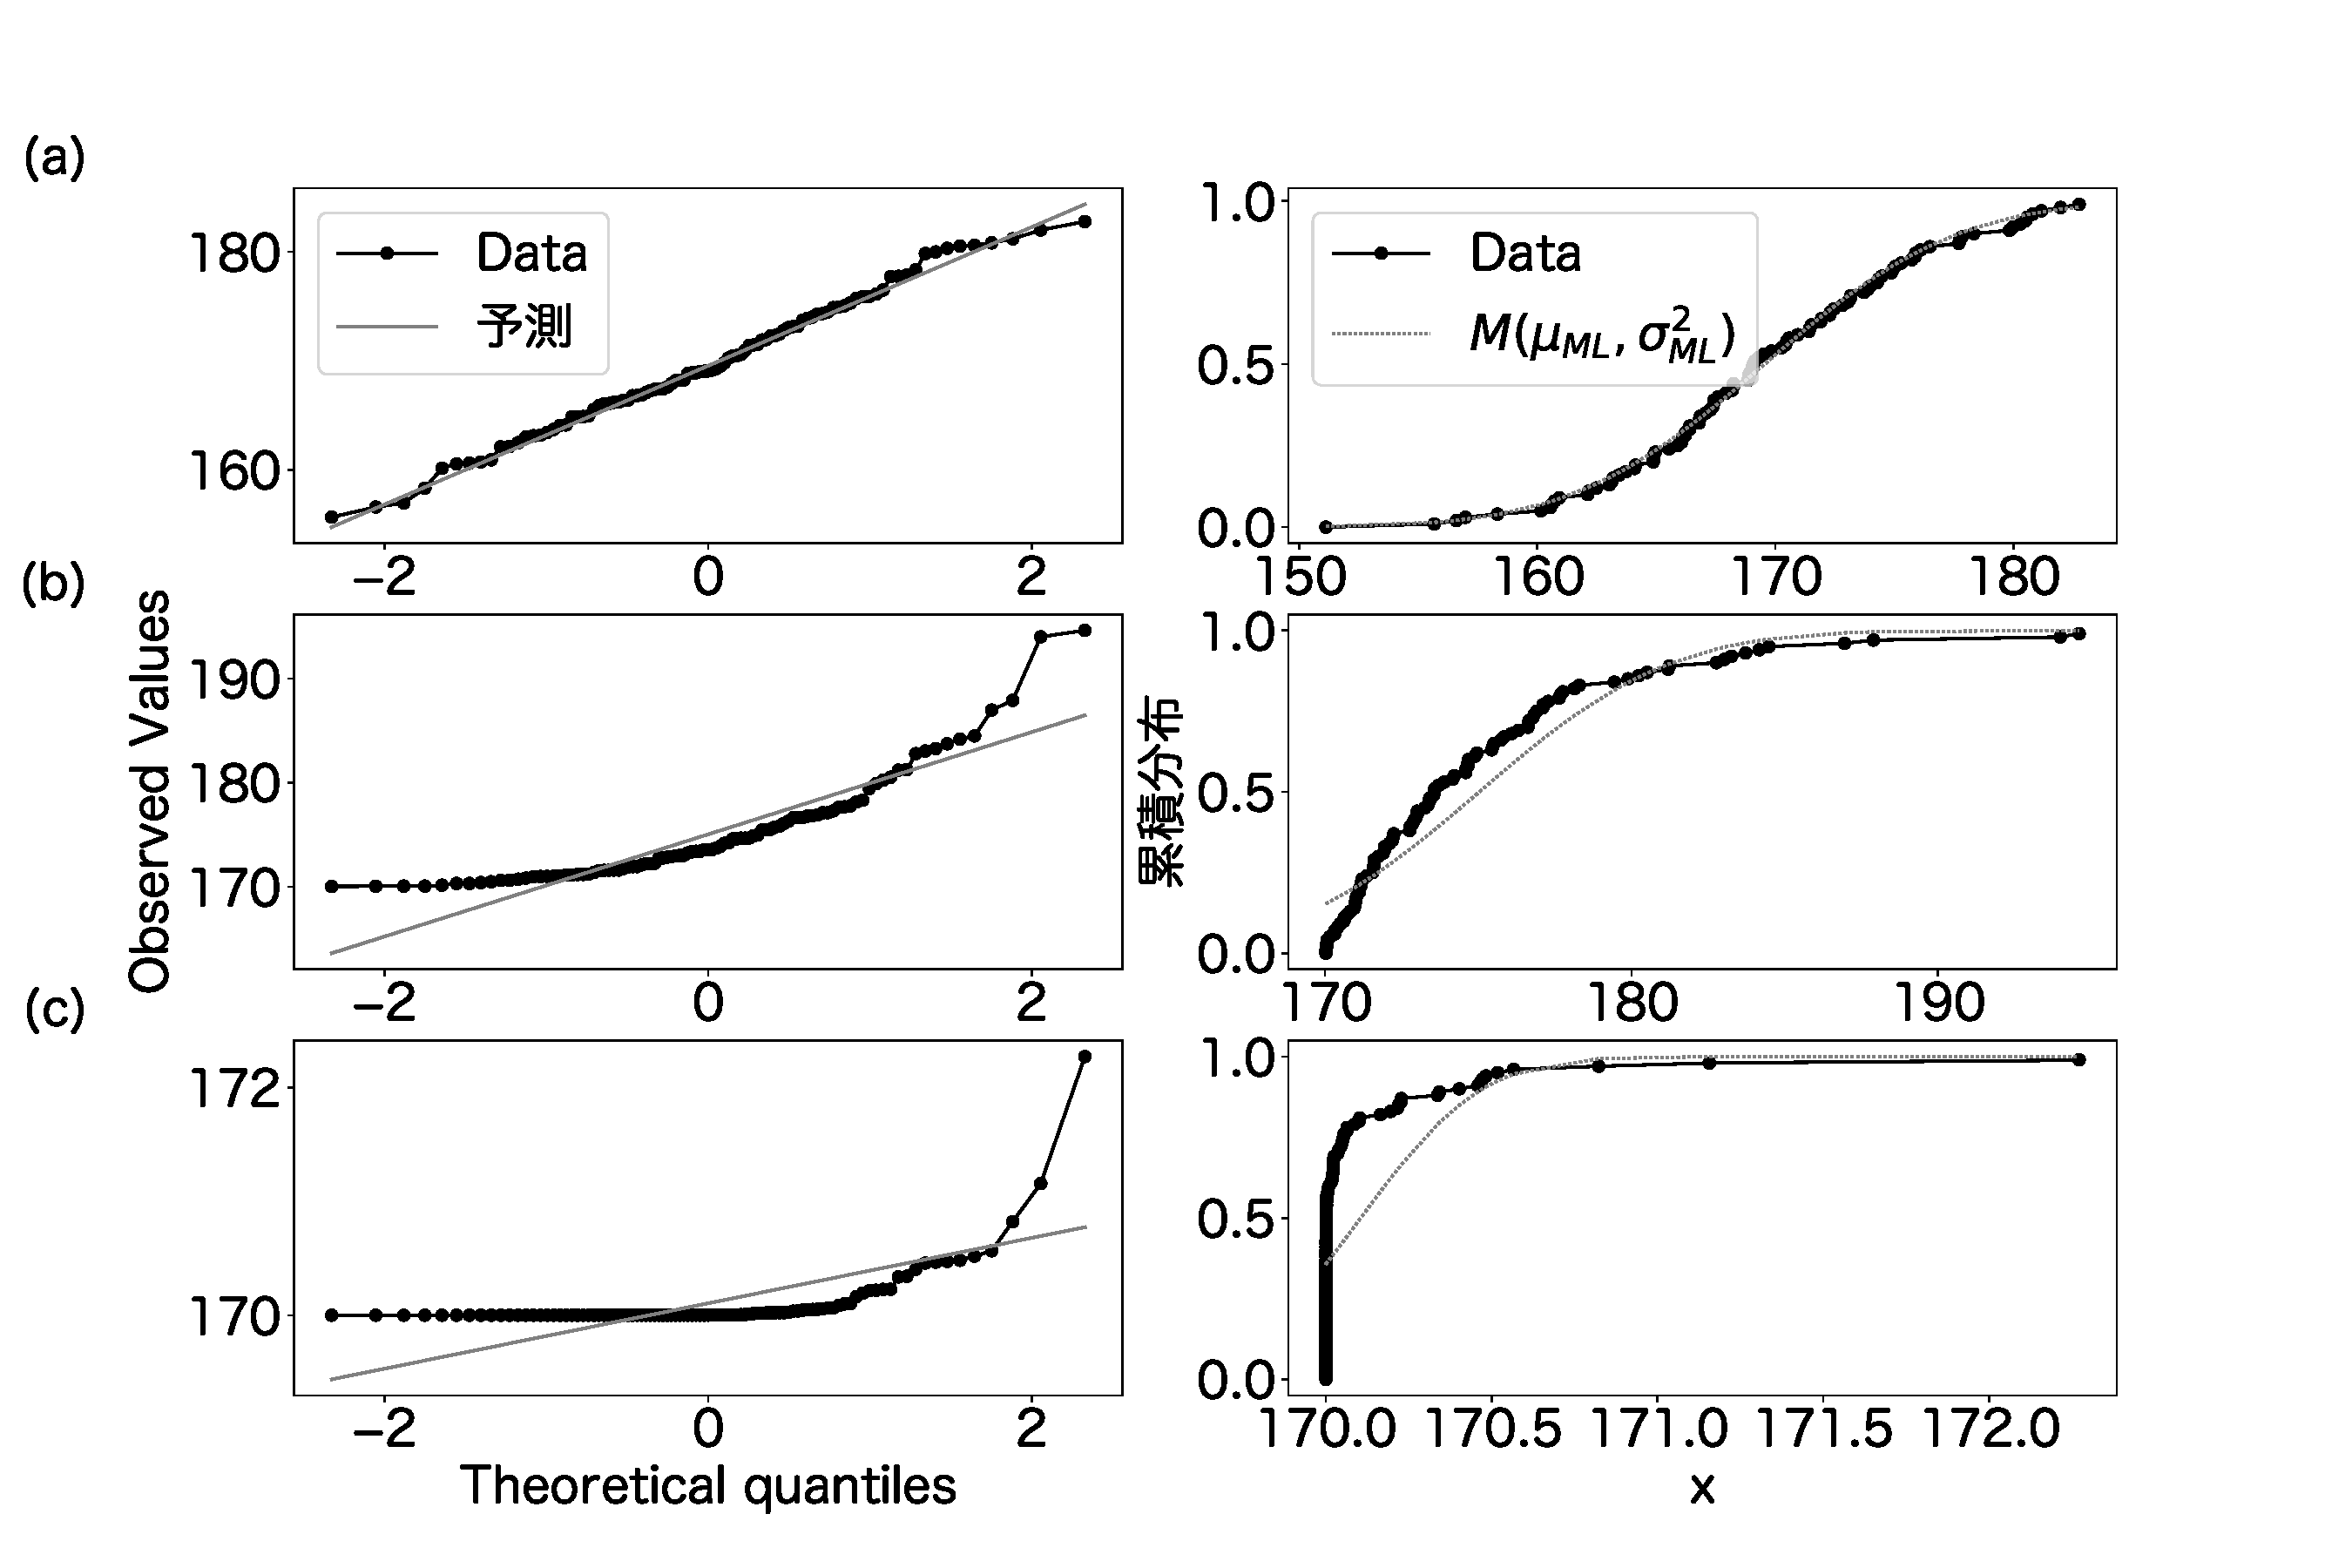
\includegraphics[width=15cm]{./image/12_/qq_cummlative_expon_norm_gamma.pdf}
        \label{fig:qq_cummlative}
        \caption{左にはqqプロット、右は累積分布と最尤モデルの累積分布。サンプルサイズは100(a)正規分布$N(170,5.8)$(b)指数分布$\lambda=5.8$(c)ガンマ分布$s=0.1$)}
    \end{center}
\end{figure}

\begin{figure}
    \begin{center}
        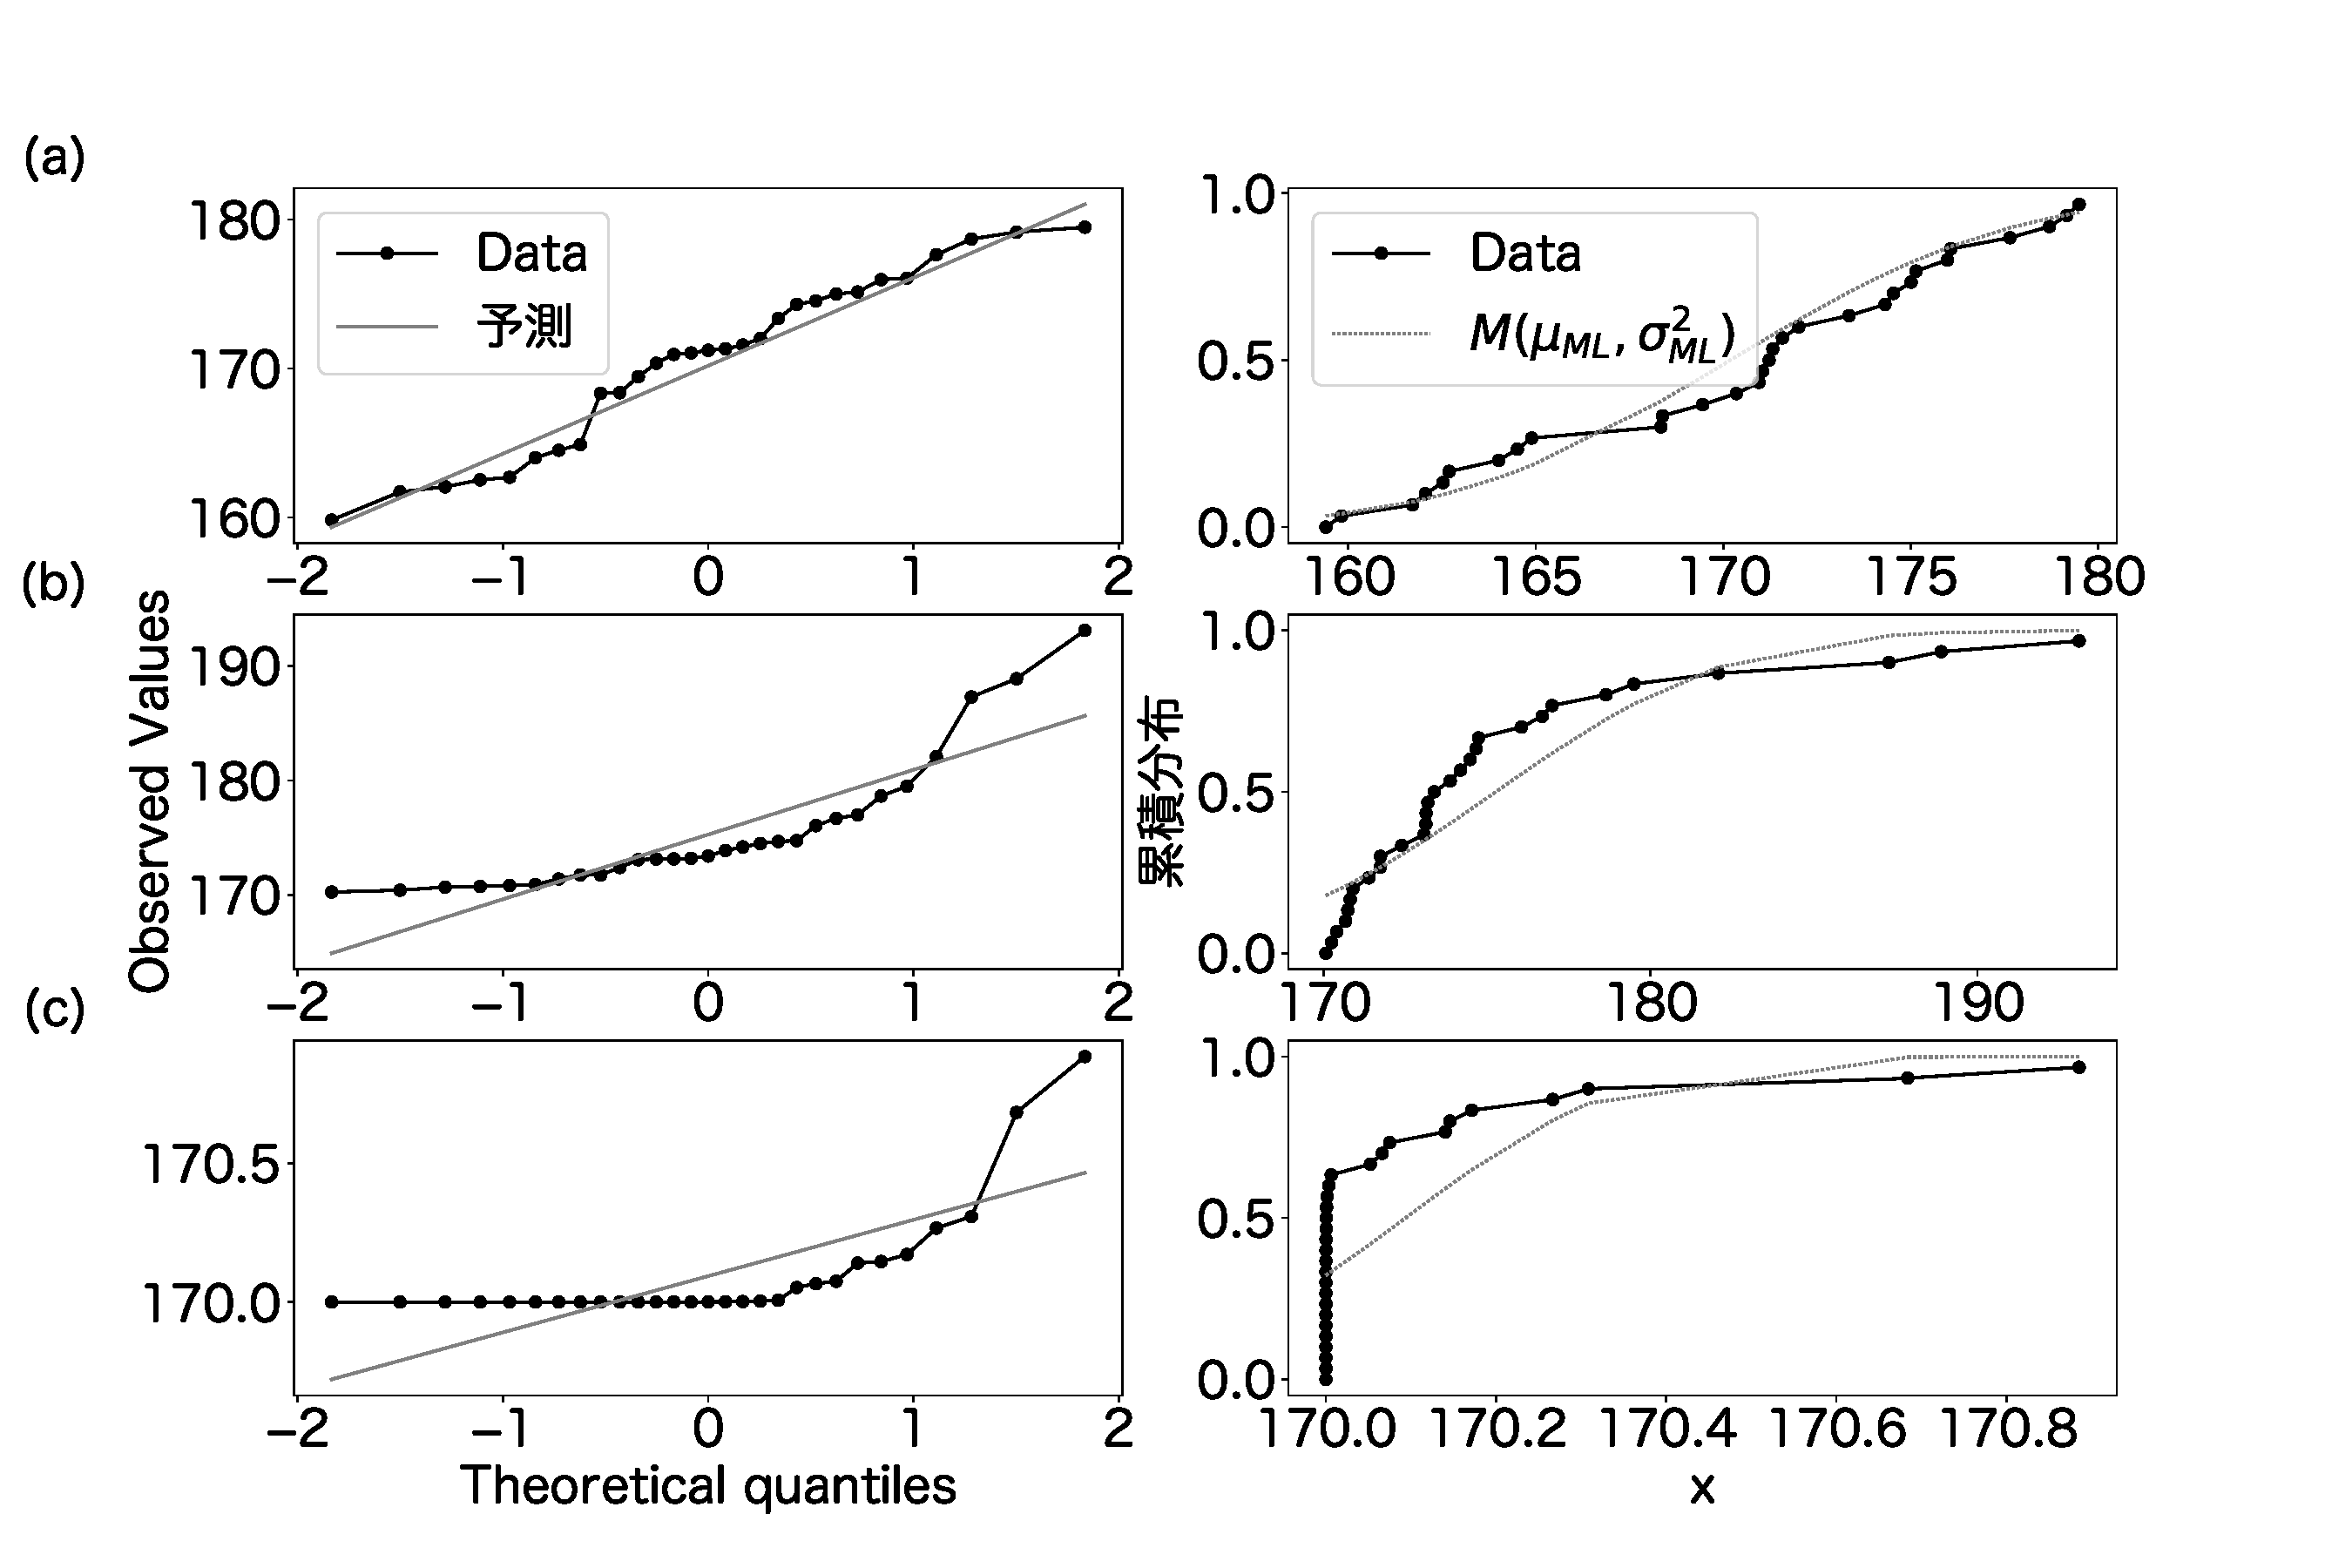
\includegraphics[width=15cm]{./image/12_/qq_cummlative_expon_norm_gammaN_30.pdf}
        \label{fig:qq_cummlative_30}
        \caption{左にはqqプロット、右は累積分布と最尤モデルの累積分布。サンプルサイズは30(a)正規分布$N(170,5.8)$(b)指数分布$\lambda=5.8$(c)ガンマ分布$s=0.1$)}
    \end{center}
\end{figure}


\subsection{AICの比較}
AICは、対数尤度に対して、データ由来のパラメータ分、ペナルティを与えたものである。
AICが低いモデルは、相対的に良くデータに当てはまるモデルであり、そのモデルからデータが生成されたことを示唆するものではない。また、AICの差が$10$あったから良いとか悪いとかではなく、AICが低いものが相対的に良いモデルと判断されがちになるだけである。AICが小さいから、良い予測をするということは一般にない。

正規モデルのデータに対するAICを計算する。
母数を最尤推定により決定した最尤モデルのパラメータ数は2である\footnote{データ由来の母数2つあるので}。
過去の研究データから、平均$\mu$を決定し分散については最尤推定量により決定したモデル$M(\sigma^2_{ML})$のパラメータ数は$1$である。

\subsubsection{AICが低いモデルは良い予測をするモデル?}
AICが低いから、良い予測ができるかは不明である。
一般に、比較対象のモデルの中で、データへの適合度が相対的に高いモデルである。
まず、AICが低いモデルでも、データの出現を予測しにくい事例を紹介する。





\section{モデルでデータを推測可能}
\subsection{ひとつのデータから推測する}
サンプルサイズ$1$の標本が正規モデル$M(\mu)$により予測できるのかを考える。
$M(\mu)$であれば、$95\%$の確率で、$\mu-\sigma z_{0.025}\sim \mu-\sigma z_{0.025}$の間でデータが見つかることを予測する。
この中に入っていることが予測可能の目安の一つにはなる。

サンプルサイズが小さい場合では、標本分布の形がどの分布に適合するのかを推測しにくので、このモデルが現実を予測していると言い切ることはできない。

%我々の科学では、モデルが現象を推測可能であるかをたったひとつの値から判定しない。

%$\sigma^2=1$とすると、$95\%$の確率で、確率変数は、$\mu-1.96\sim\mu+1.96$の間で見つかる。
%$\mu=0$なら、$x=0.1$は、この区間の中にあるので、$x$は、$N(0,1)$では良く見つかる値になる。
%この基準では、複数の$\mu$で$x=0.1$はよく見つかる範囲に入る。例えば、$\mu=0.1$でも良く確率変数が見つかる区間は、$-1.85\sim 2.05$なので、確率変数は、$N(0.1,1)$に従うとしても問題ない。
%$x=0.1$がその区間に入らない母数は、$\mu=z_{0.025}+0.1$のときで、区間は$0.10003\sim4.01$で、この区間に$x$は入ってません。
%これを言い換えれば、母数$x-z_{0.025}\leq\mu\leq x+z_{0.025}$の間でよくある値になり、この間から外れた母数をもつ$N(\mu,1)$に従っていいないと推測できる。

\if 0
例えば、$x=1.97$が得られたとすると、$N(0,1)$のよく出る値の範囲は、$-1.96\sim1.96$であることから、母数$0$ではないと判断できます。
一方で、$N(0,1)$で$x=1.97$は、サンプルサイズが$20$であれば、そのうち$1$回は、$1.97$をとる値です。もしももう一度サンプリングできたとして、その値が$0$になることもあり得ます。
以上のことから、$1$回のサンプリングだけで判断しません。
\fi


